\documentclass[12pt,a4paper]{article}
\title{Lab4-Lucene1(构建搜索引擎)}
\usepackage{ctex}
\usepackage{amsmath,amscd,amsbsy,amssymb,latexsym,url,bm,amsthm}
\usepackage{epsfig,graphicx,subfigure}
\usepackage{enumitem,balance}
\usepackage{wrapfig}
\usepackage{mathrsfs,euscript}
\usepackage[usenames]{xcolor}
\usepackage{hyperref}
\usepackage[vlined,ruled,commentsnumbered,linesnumbered]{algorithm2e}
\usepackage{float}
\usepackage{geometry}
\usepackage{listings}
\geometry{a4paper,scale=0.8}
\usepackage[T1]{fontenc}
\usepackage[utf8]{inputenc}
\usepackage{amssymb}
% --- Python code template ---
\usepackage[utf8]{inputenc}
% Default fixed font does not support bold face
\DeclareFixedFont{\ttb}{T1}{txtt}{bx}{n}{12} % for bold
\DeclareFixedFont{\ttm}{T1}{txtt}{m}{n}{12}  % for normal

% Custom colors
\usepackage{color}
\definecolor{deepblue}{rgb}{0,0,0.5}
\definecolor{deepred}{rgb}{0.6,0,0}
\definecolor{deepgreen}{rgb}{0,0.5,0}

\usepackage{listings}

% Python style for highlighting
\newcommand\pythonstyle{\lstset{
language=Python,
basicstyle=\ttm,
morekeywords={self},              % Add keywords here
keywordstyle=\ttb\color{deepblue},
emph={MyClass,__init__},          % Custom highlighting
emphstyle=\ttb\color{deepred},    % Custom highlighting style
stringstyle=\color{deepgreen},
frame=tb,                         % Any extra options here
showstringspaces=false
}}
% Python environment
\lstnewenvironment{python}[1][]
{
\pythonstyle
\lstset{#1}
}
{}

% Python for external files
\newcommand\pythonexternal[2][]{{
\pythonstyle
\lstinputlisting[#1]{#2}}}

% Python for inline
\newcommand\pythoninline[1]{{\pythonstyle\lstinline!#1!}}

% --- Python code template ---


\title{Lab4\quad Lucene1(构建搜索引擎)}
\date{2021.10}
\author{孙济宸\quad \quad 学号:520030910016 \quad  \quad 班级:F2003003}
\begin{document}
\maketitle
\section{实验概览}
\begin{enumerate}
	\item 对Lab3中爬虫获取的大量中文网页进行\textbf{索引},修改IndexFiles.py,将每个网页的\textbf{文件名、存储地址、URL、标题和文本内容}索引化;
	\item 运用\textbf{jieba}分词对网页文本\textbf{分词},方便使用WhitespaceAnalyzer索引和查找;
	\item 修改SearchFiles.py实现搜索,显示搜索结果的\textbf{文件名、存储地址、URL、标题和文本内容}。
\end{enumerate}
\section{实验环境}
\begin{itemize}
	\item Docker
	\item \textbf{beautifulsoup (bs4)}
	\item \textbf{pylucene}
	\item \textbf{jieba}
	\item \textbf{paddle}: jieba启用paddle功能依赖库;需运行pip install paddlepaddle
	\item re (正则表达式)
	\item os

\end{itemize}
\newpage

\section{练习题的解决思路}
\subsection{问题1-IndexFiles建立索引}
\subsubsection{对爬虫的修改} \label{addhtml}
由于在建立索引时需要在doc的field中加入网页的URL,方便查询时显示网页链接,但是个人认为,在添加索引时查询index.txt带来额外性能开销,而且.html文件名不能更改,否则查找不到对应的url。
\\因此我的做法是在爬取网页时将网页自己的URL在爬取完将要写入文件前,\textbf{在html文件头上写入网页本身的URL},这样建立索引时读取.html文件时可直接从文件中获取自身的URL。
\begin{python}
SELF_URL_MARKER  = "SELF_URL_TAG:"
f = open(os.path.join(folder, filename), 'w',encoding='utf-8')
f.write("<!- "+SELF_URL_MARKER + page + " -->" + "\n")  
#写html加入含有自身URL的注释
f.write(str(content))
f.close()
\end{python}
\begin{figure}[H]
	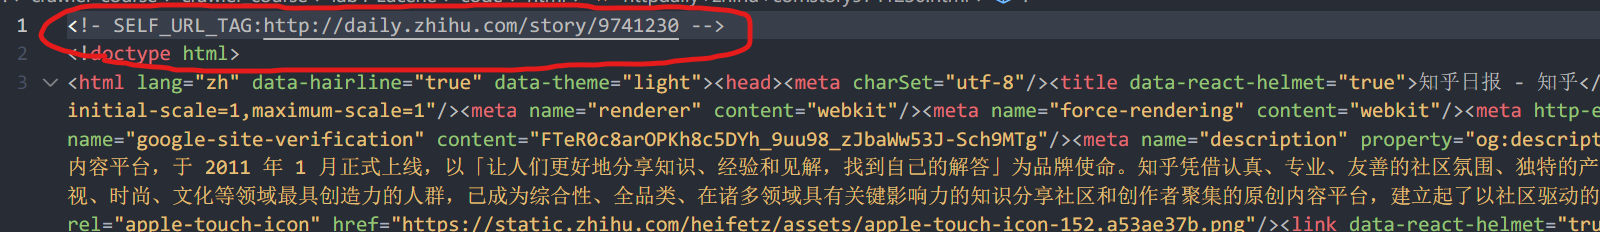
\includegraphics[width=\textwidth]{selftag.png}
	\centering
	 \caption{含有网页自身URL的自定义注释标签}
\end{figure}
\subsubsection{建立索引}
从目录中读取html文件后,
\begin{itemize}
\item 文件名、文件路径直接从os中获取;
\item title通过BeautifulSoup解析<title><\textbackslash title>标签获取  ( get{\_}self{\_}url(content) )
\item URL通过正则表达式,匹配\ref{addhtml}中添加的自定义注释标签获取。 ( get{\_}title(content) )
\item 文本内容通过clean{\_}html(content)函数去除内嵌代码和html标签后,使用jieba库的cut{\_}for{\_}search()函数进行分词,最终获取\textbf{空格分隔的纯文字内容}(contents);
\item 将name, path, title, URL, contents加入doc的Field中。其中前四者类型为t1(存储,不索引),contents为t2(不存储但索引)。
\item 使用WhitespaceAnalyzer,建立索引。

\end{itemize}
\subsection{实现搜索}
对用户输入的搜索词,使用与索引时相同的jieba.cut{\_}for{\_}search()函数和WhitespaceAnalyzer,经过QueryParser处理搜索词(QueryParser能够处理布尔运算符)后,使用searcher搜索。得到结果并输出每个结果的path, filename, score, URL 和 title.

\section{代码运行结果}
\subsection{建立索引}
运行IndexFiles{\_}zhCN.py
\begin{figure}[H]
	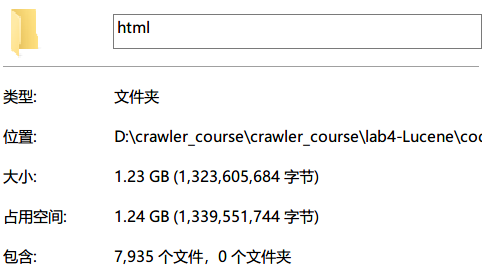
\includegraphics[width=0.7\textwidth]{htmls.png}
	\centering
	 \caption{html}
\end{figure}
\begin{figure}[H]
	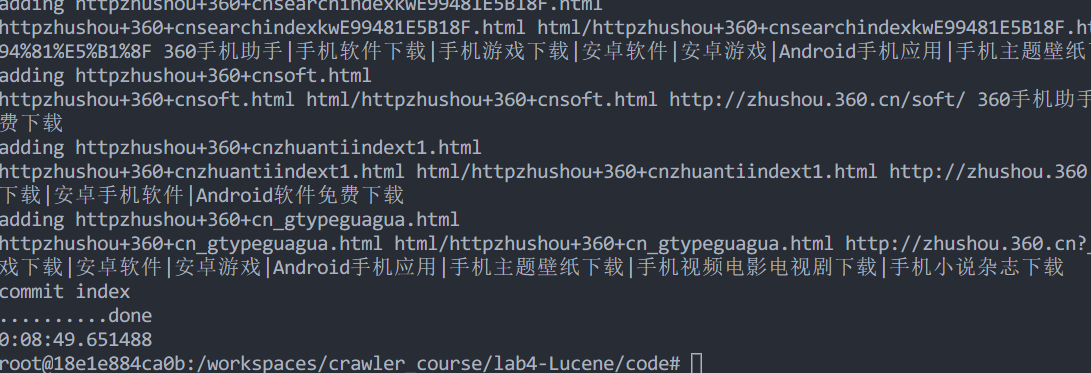
\includegraphics[width=0.7\textwidth]{indexed.png}
	\centering
	 \caption{IndexFiles{\_}zhCN.py}
\end{figure}
\begin{figure}[H]
	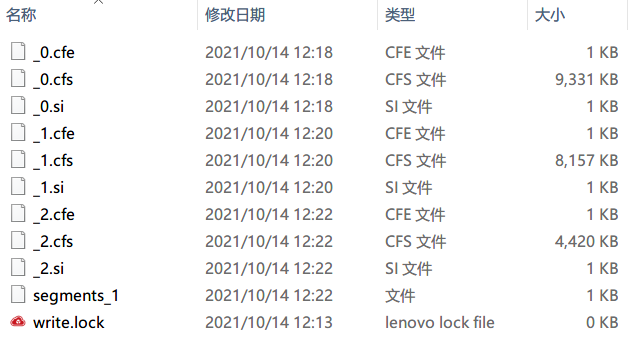
\includegraphics[width=0.7\textwidth]{indexfolder.png}
	\centering
	 \caption{index{\_}zhCN}
\end{figure}



\subsection{搜索}
运行SearchFiles{\_}zhCN.py进行搜索
\subsubsection{query a-故意找茬}
\begin{figure}[H]
	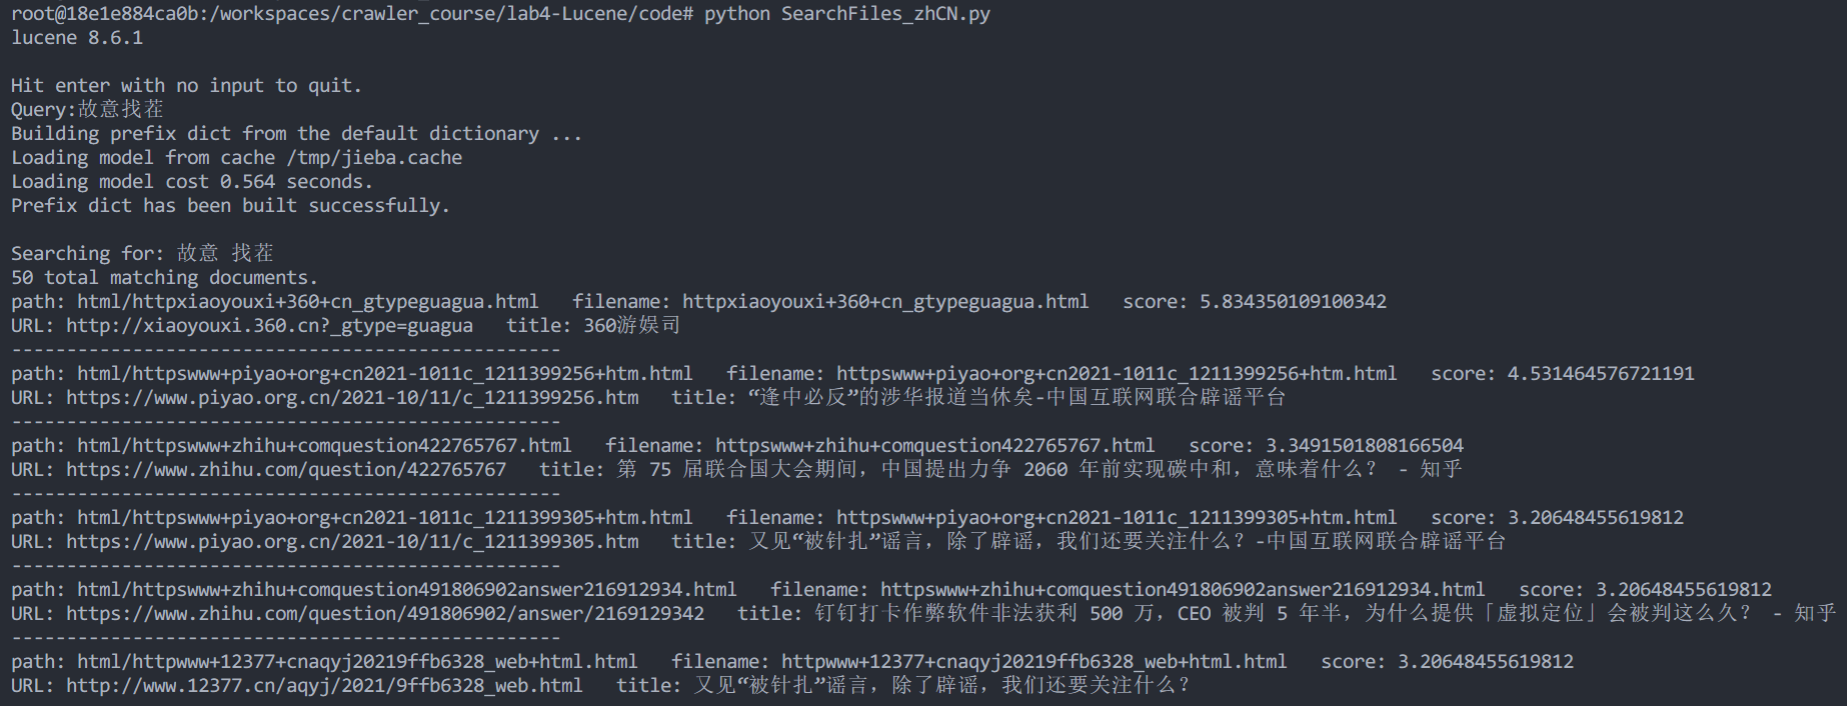
\includegraphics[width=\textwidth]{query1.png}
	\centering
	
\end{figure}

\subsubsection{query b-苹果手机}
\begin{figure}[H]
	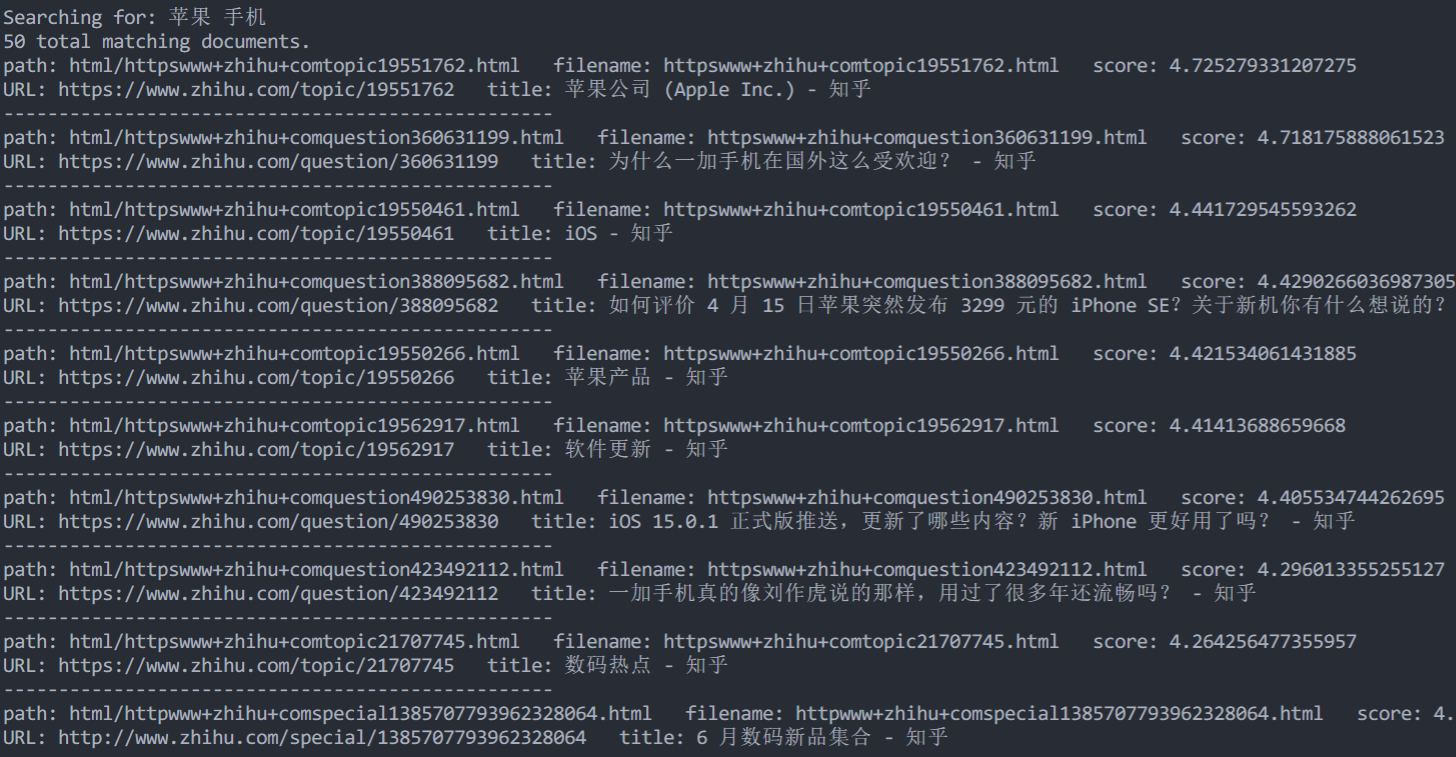
\includegraphics[width=\textwidth]{query2.png}
	\centering
\end{figure}

\begin{figure}[H]
	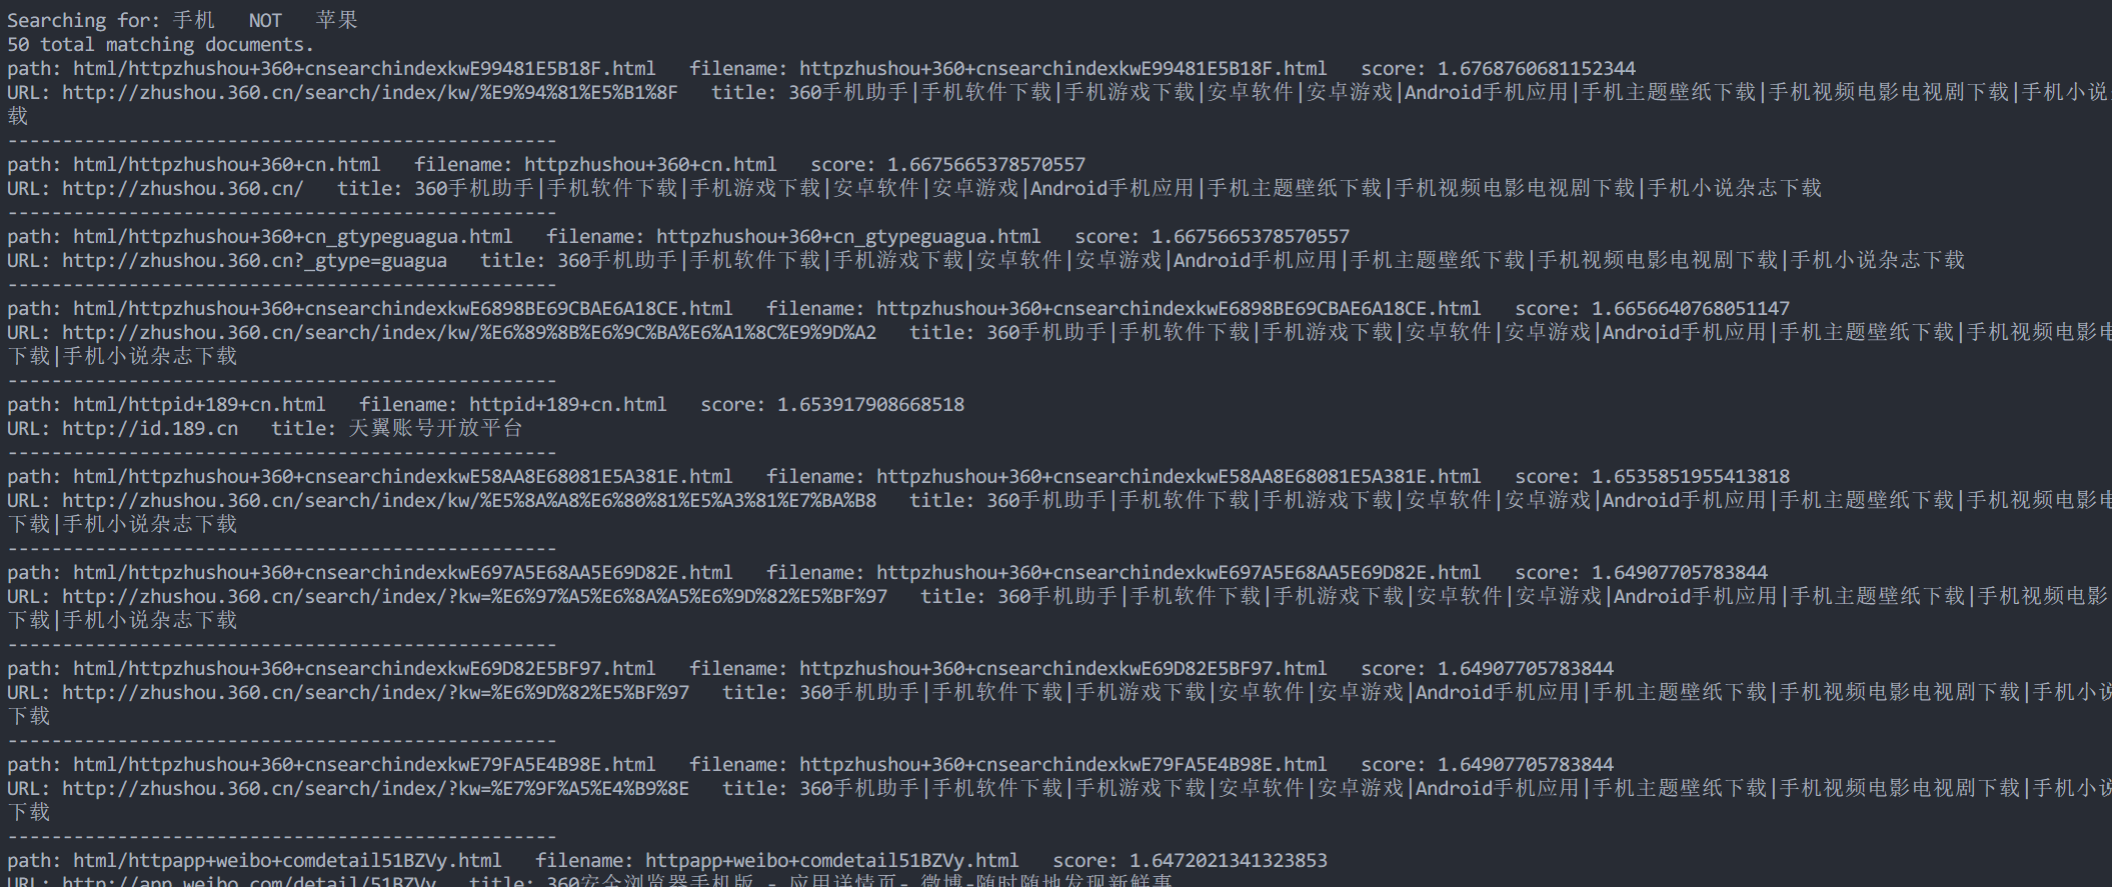
\includegraphics[width=\textwidth]{query3.png}
	\centering
\end{figure}

\begin{figure}[H]
	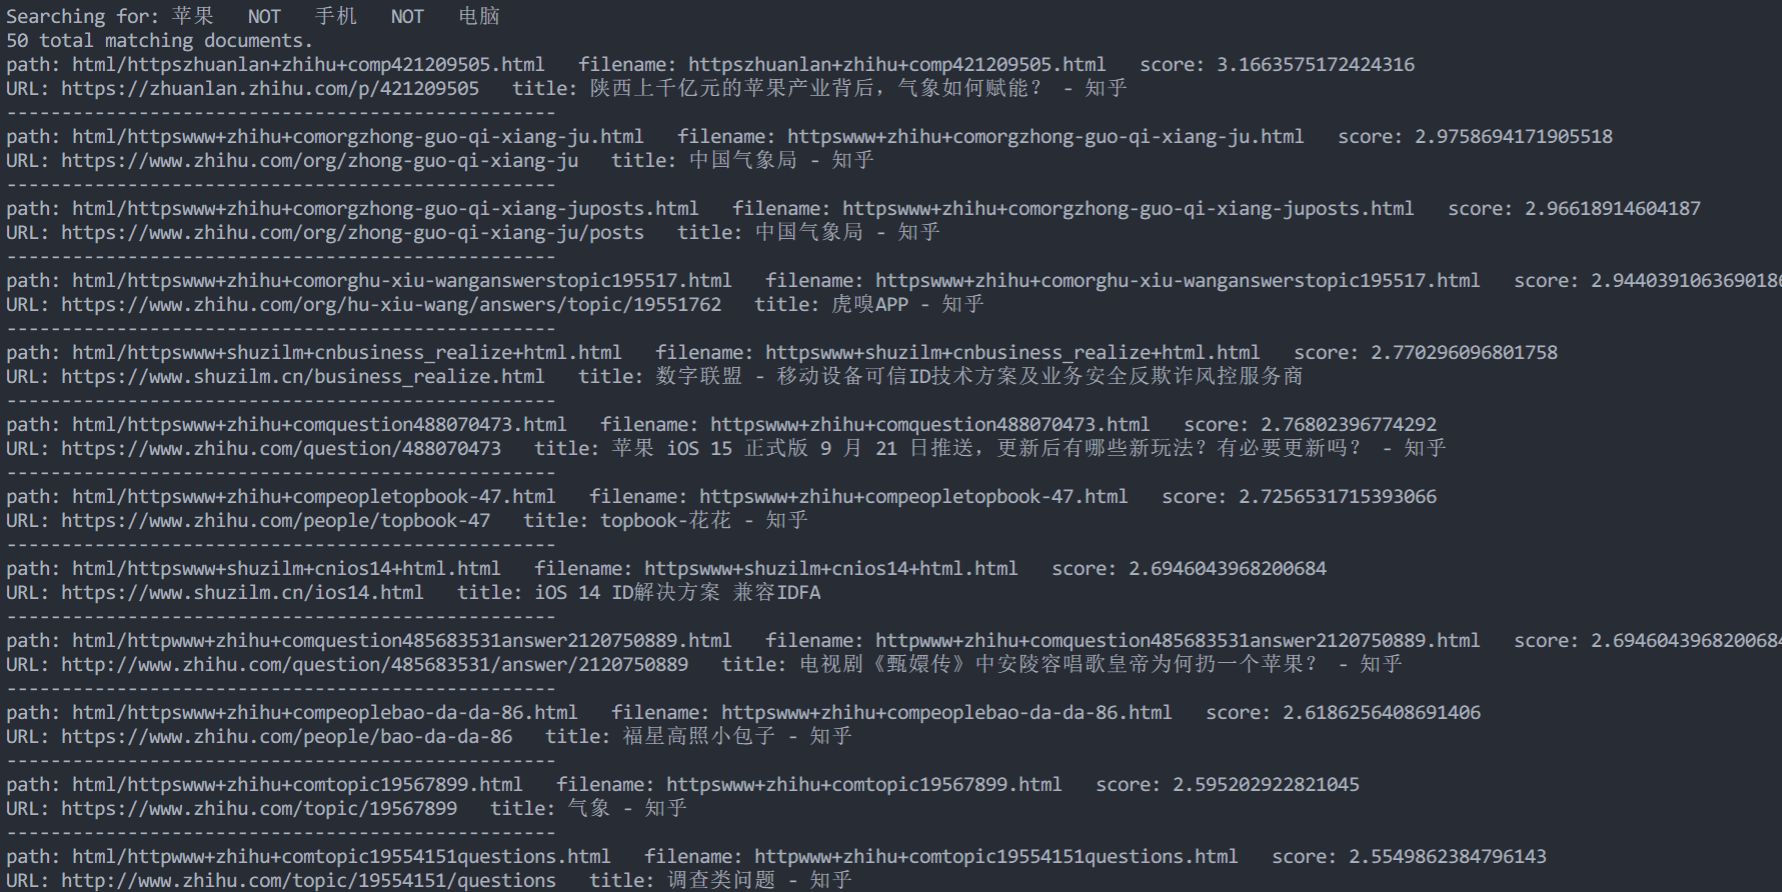
\includegraphics[width=\textwidth]{query4.png}
	\centering
\end{figure}

\subsubsection{query c-美国俄罗斯}
\begin{figure}[H]
	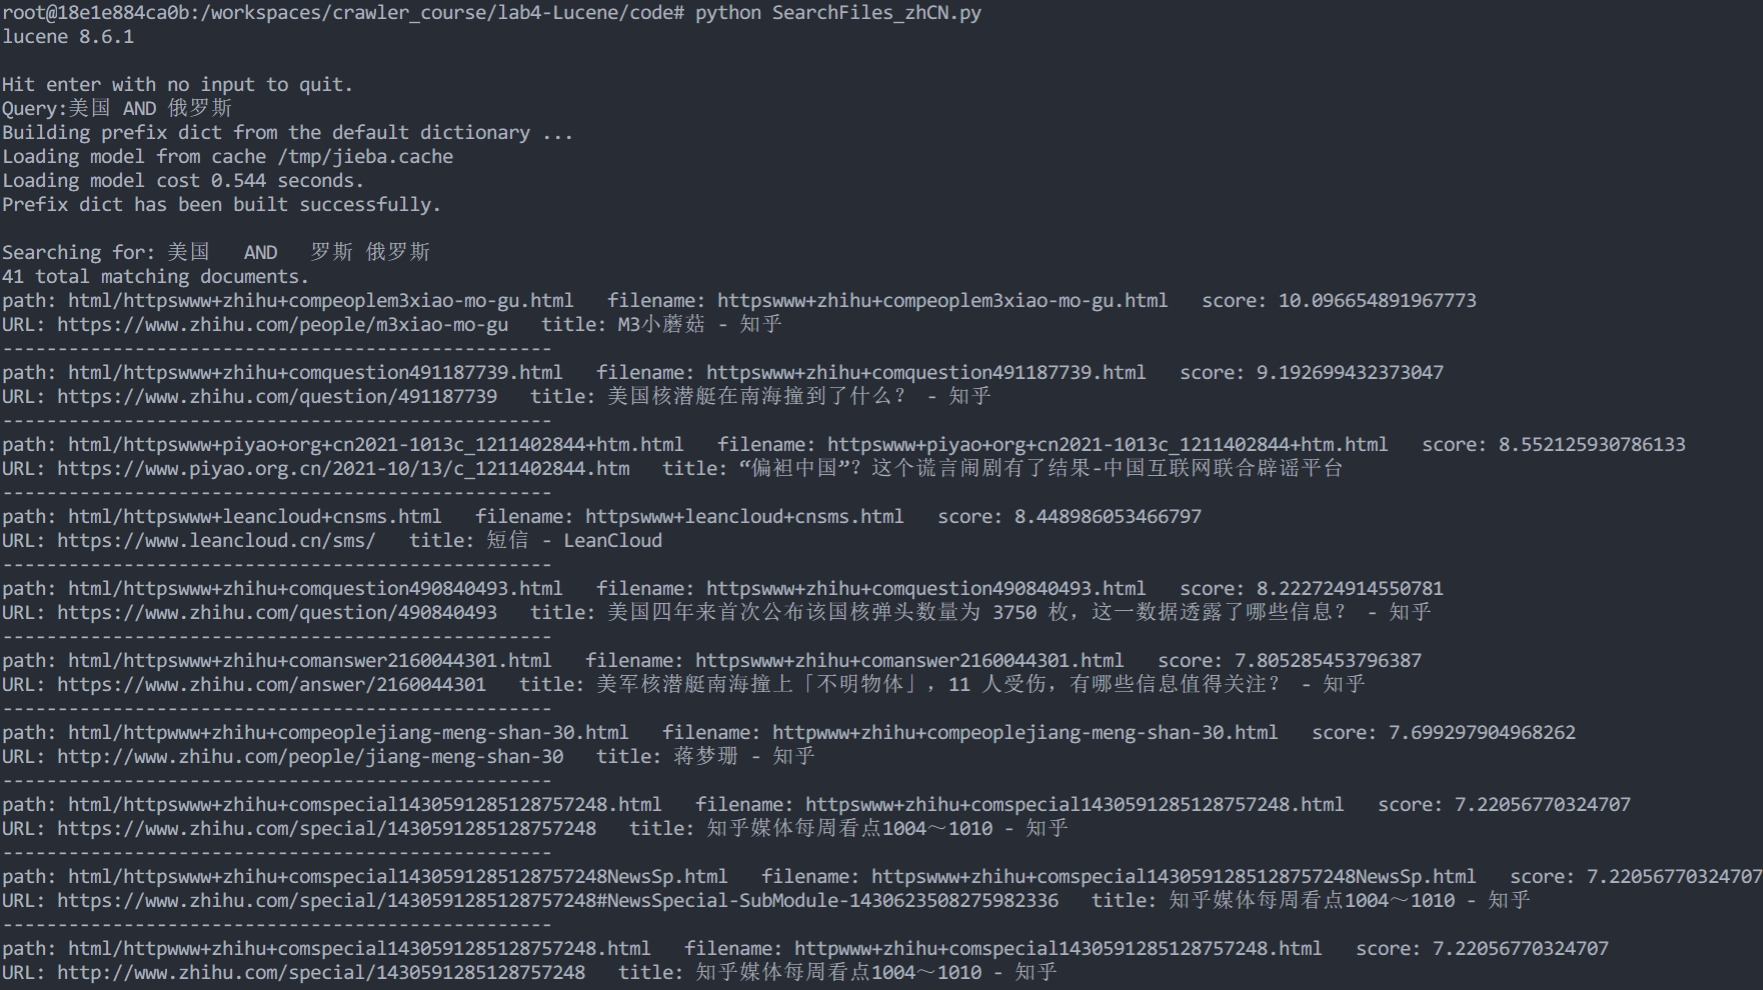
\includegraphics[width=\textwidth]{query5.png}
	\centering
\end{figure}

\subsubsection{query d-腾讯官司}
\begin{figure}[H]
	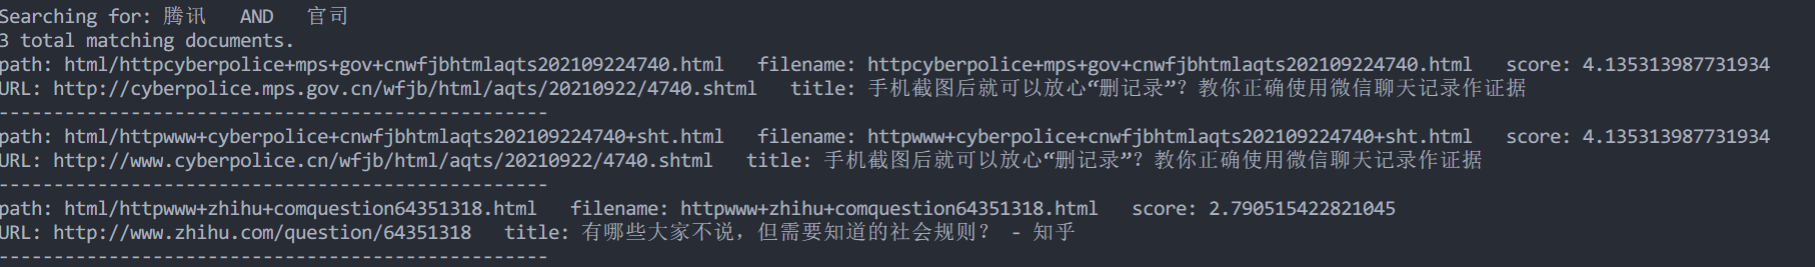
\includegraphics[width=\textwidth]{query6.png}
	\centering
\end{figure}

\begin{figure}[H]
	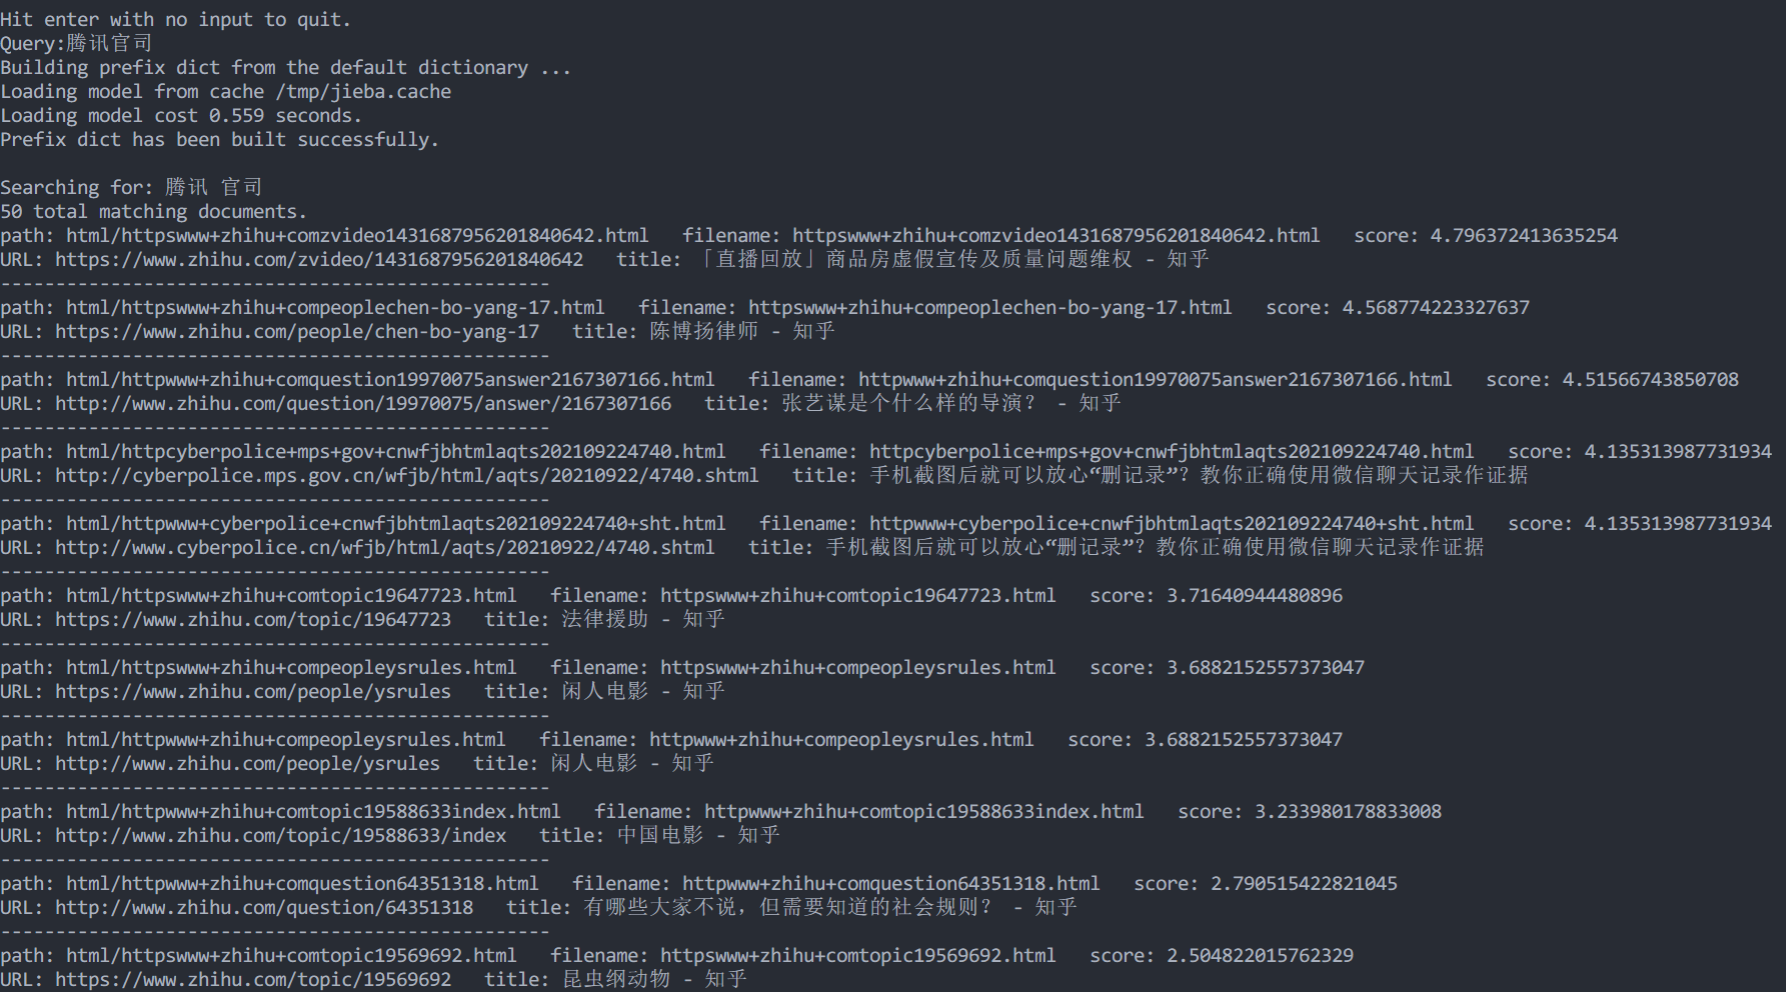
\includegraphics[width=\textwidth]{query7.png}
	\centering
\end{figure}

\section{分析与思考}
\begin{itemize}
	\item 在jieba分词完成后不能使用pylucene的StandardAnalyzer,因为它会将中文单词一个一个字拆开分析,而是应该使用WhitespaceAnalyzer。
	\item 通过尝试发现,jieba库的cut{\_}for{\_}search()对于构建索引和搜索效果最好,它会将长词的多种分词方法都加入分词结果。同时启用推荐的paddle模块(深度学习分词)能提升分词准确度。 最后经过手动验证,实现搜索的相关性比较高。
	\item 建立索引时,处于性能和实现难易度考虑我选择在爬虫中把网页自身URL写在html文件里,而不是在index.txt中查询
	\item 搜索时,需要使用与构建索引时相同的分词和Analyzer。
\end{itemize}

\end{document}

